%!TEX program = xelatex

\documentclass[UTF8]{ctexart}
\usepackage{ctex}

\CTEXsetup[format={\Large\bfseries}]{section}

\usepackage[version=3]{mhchem} % Package for chemical equation typesetting
\usepackage{siunitx} % Provides the \SI{}{} and \si{} command for typesetting SI units
\usepackage{graphicx} % Required for the inclusion of images
\graphicspath{{assets/}}
\usepackage{natbib} % Required to change bibliography style to APA
\usepackage{amsmath} % Required for some math elements 
\usepackage{amssymb}
\usepackage[hidelinks]{hyperref}
\usepackage{makecell} % 3 Packages for flexible tabular
\usepackage{multirow}
\usepackage{multicol}

\usepackage{geometry}% 版面大小
\geometry{a4paper,scale=0.7}

\usepackage{fontspec}

\setCJKfamilyfont{hwxk}{STXingkai}% 字体
\newcommand{\hwxk}{\CJKfamily{hwxk}}

\usepackage{fancyhdr}% 页眉页脚
\fancypagestyle{EE_AnalogExp_template}{
    \fancyhead[L]{\Large {\hwxk 南京大学电子科学与工程学院}}
    \fancyhead[R]{数字系统1实验报告}
    \fancyfoot[c]{- \thepage \ -}
    \renewcommand\footrulewidth{0pt}
}

% 4级目录
\setcounter{secnumdepth}{4}
\setcounter{tocdepth}{4}

\usepackage{graphicx} % Packages for figures
\usepackage{caption2}
\usepackage{subfigure}
\usepackage{float}


%设置图片、表格编号
\renewcommand{\thetable}{\thesubsection{}-\arabic{table}}
\renewcommand{\thefigure}{\thesubsection{}-\arabic{figure}}
\renewcommand{\thefigure}{\thesubsection{}-\arabic{equation}}
\usepackage{amsmath}
\numberwithin{figure}{subsection}
\numberwithin{table}{subsection}
\numberwithin{equation}{subsection}

\setlength\parindent{6pt} % Removes all indentation from paragraphs

\renewcommand{\labelenumi}{\alph{enumi}.} % Make numbering in the enumerate environment by letter rather than number (e.g. section 6)

%\usepackage{times} % Uncomment to use the Times New Roman font

%----------------------------------------------------------------------------------------
%	DOCUMENT INFORMATION
%----------------------------------------------------------------------------------------

\title{\textbf{实验1\ 组合逻辑电路}} % Title

\author{电子科学与工程学院 刘时宜} % Author name

\date{} % Date for the report

\begin{document}

\pagestyle{EE_AnalogExp_template}

\maketitle % Insert the title, author and date

\begin{center}
    \begin{tabular}{l r}
    实验日期: & 2021年10月26日 \\ % Date the experiment was performed
    指导老师: & 高健 % Instructor/supervisor
    \end{tabular}
    \par 点击目录、书签栏、以及行文中的图表标号的均可跳转至相应页面
    \end{center}
    
% If you wish to include an abstract, uncomment the lines below
% \begin{abstract}
% Abstract text
% \end{abstract}

\tableofcontents

\section{实验目的}
\begin{enumerate}
    \item 熟悉开发板的使用
    \item 测试并验证组合逻辑电路
\end{enumerate}

\section{实验仪器与主要器材}
\begin{center}
    \begin{tabular}{ll}
        \textbf{仪器:} & \\
        Basys3 FPGA 开发板 & 1台\\
        KEYSIGHT DSOX1102AG 示波器 & 1台\\
        示波器高频探头 & 1套\\
        ROGOL DM3068 万用表 & 1台\\
        \textbf{软件:} & \\
        Multisim & 14.1 \\
        Digilent Adept & 2.19.2 \\
        Vivado & 2015.4 \\
        \textbf{耗材:} & \\
        导线 & 若干 \\
    \end{tabular}
\end{center}

\section{实验原理}
\par 组合逻辑电路在逻辑功能上的特点是任一时刻的输出仅仅取决于该时刻的输入,与电路的原来的状态无关。
\par FPGA(Field-Programmable-Gate-Array,现场可编程逻辑门阵列)是一种可以通过软件编程,实现自定义逻辑功能的芯片。

\section{实验过程}
\subsection{测量并验证组合逻辑电路}
\subsubsection{实验内容}
\par 通过四个与非门实现异或逻辑,观察并测量输入、中间点和输出点各逻辑状态。电路逻辑等效电路如图\ref{logic eqiv circuit}所示。改变\(S_0\)、\(S_1\)的逻辑状态,测试电路在不同脉冲方波信号下电路的输出。

\begin{figure}[H]
    \begin{center}
        \includegraphics[width=0.8\textwidth]{equiv cirvuit.jpg}
    \end{center}
    \caption{逻辑等效电路}
    \label{logic eqiv circuit}
\end{figure}

\subsubsection{实验数据}
\paragraph{\(S_0  = S_1 = 0\)}~
\par 实验结果如表\ref{00 pic}所示,实验数据如表\ref{00 data}所示。

\begin{figure}[H]
    \centering
    \subfigure[A=0, B=0]{
    \includegraphics[width=0.35\textwidth]{00/00.png}}
    \subfigure[A=0, B=1]{
    \includegraphics[width=0.35\textwidth]{00/01.png}}
    \subfigure[A=1, B=0]{
    \includegraphics[width=0.35\textwidth]{00/10.png}}
    \subfigure[A=1, B=1]{
    \includegraphics[width=0.35\textwidth]{00/11.png}}

    \caption{\(S_0  = S_1 = 0\)时不同输入下电路情况}
    \label{00 pic}
\end{figure}

\begin{table}[h]
    \begin{center}
        \begin{tabular}{|c|c|c|c|c|c|}
            \hline
            A & B & \(Z_0\) & \(Z_1\) & \(Z_2\) & \(Z_3\) \\
            \hline
            0 & 0 & 0 & 1 & 1 & 1 \\
            \hline
            1 & 0 & 1 & 1 & 1 & 0 \\
            \hline
            0 & 1 & 1 & 1 & 0 & 1 \\
            \hline
            1 & 1 & 0 & 0 & 1 & 1 \\
            \hline
        \end{tabular}
        \caption{\(S_0  = S_1 = 0\)时的实验数据}
    \end{center}
    \label{00 data}
\end{table}

\paragraph{\(S_1 = 0 ,S_0 = 1, A = 0\)}~
\par 实验数据如图\ref{010 pic}所示。各图中黄线(通道1)为B, 绿线(通道2)为测量端口.

\begin{figure}[H]
    \centering
    \subfigure[\(JB_0\)]{
    \includegraphics[width=0.35\textwidth]{010/jb0.jpg}}
    \subfigure[\(JB_1\)]{
    \includegraphics[width=0.35\textwidth]{010/jb1.jpg}}
    \subfigure[\(JB_2\)]{
    \includegraphics[width=0.35\textwidth]{010/jb2.jpg}}
    \subfigure[\(JB_3\)]{
    \includegraphics[width=0.35\textwidth]{010/jb3.jpg}}
    \subfigure[\(A\)]{
    \includegraphics[width=0.35\textwidth]{010/a.jpg}}

    \caption{\(S_1 = 0 ,S_0 = 1, A = 0\)电路各引脚波形}
    \label{010 pic}
\end{figure}

\paragraph{\(S_1 = 0 ,S_0 = 1, A = 1\)}~
\par 实验数据如图\ref{011 pic}所示。各图中黄线(通道1)为B, 绿线(通道2)为测量端口.

\begin{figure}[H]
    \centering
    \subfigure[\(JB_0\)]{
    \includegraphics[width=0.35\textwidth]{011/jb0.jpg}}
    \subfigure[\(JB_1\)]{
    \includegraphics[width=0.35\textwidth]{011/jb1.jpg}}
    \subfigure[\(JB_2\)]{
    \includegraphics[width=0.35\textwidth]{011/jb2.jpg}}
    \subfigure[\(JB_3\)]{
    \includegraphics[width=0.35\textwidth]{011/jb3.jpg}}
    \subfigure[\(A\)]{
    \includegraphics[width=0.35\textwidth]{011/a.jpg}}

    \caption{\(S_1 = 0 ,S_0 = 1, A = 1\)电路各引脚波形}
    \label{011 pic}
\end{figure}

\paragraph{\(S_1 = 1 ,S_0 = 0\)}~
\par 实验数据如图\ref{10 pic}所示。各图中黄线(通道1)为B, 绿线(通道2)为测量端口.

\begin{figure}[H]
    \centering
    \subfigure[\(JB_0\)]{
    \includegraphics[width=0.35\textwidth]{10/jb0.jpg}}
    \subfigure[\(JB_1\)]{
    \includegraphics[width=0.35\textwidth]{10/jb1.jpg}}
    \subfigure[\(JB_2\)]{
    \includegraphics[width=0.35\textwidth]{10/jb2.jpg}}
    \subfigure[\(JB_3\)]{
    \includegraphics[width=0.35\textwidth]{10/jb3.jpg}}
    \subfigure[\(A\)]{
    \includegraphics[width=0.35\textwidth]{10/a.jpg}}

    \caption{\(S_1 = 1 ,S_0 = 0\)电路各引脚波形}
    \label{10 pic}
\end{figure}

\paragraph{\(S_1 = 1 ,S_0 = 1\)}~
\par 实验数据如图\ref{11 pic}所示。各图中黄线(通道1)为B, 绿线(通道2)为测量端口.

\begin{figure}[H]
    \centering
    \subfigure[\(JB_0\)]{
    \includegraphics[width=0.35\textwidth]{11/jb0.jpg}}
    \subfigure[\(JB_1\)]{
    \includegraphics[width=0.35\textwidth]{11/jb1.jpg}}
    \subfigure[\(JB_2\)]{
    \includegraphics[width=0.35\textwidth]{11/jb2.jpg}}
    \subfigure[\(JB_3\)]{
    \includegraphics[width=0.35\textwidth]{11/jb3.jpg}}
    \subfigure[\(A\)]{
    \includegraphics[width=0.35\textwidth]{11/a.jpg}}

    \caption{\(S_1 = 1 ,S_1 = 0\)电路各引脚波形}
    \label{11 pic}
\end{figure}

\subsubsection{讨论与小结}
\paragraph{逻辑关系的获得} 通过逻辑表达式,可以推知\(Z_0\)、\(Z_1\)、\(Z_2\)、\(Z_3\)(即\(JB_0\)、\(JB_1\)、\(JB_2\)、\(JB_3\))对于\(A\)、\(B\)的表达式分别为:

\begin{align*}
    Z_1 & = \overline{AB} \\
    Z_2 & = \overline{\overline{AB} \cdot A} = AB + \overline{A} \\
    Z_3 & = \overline{\overline{AB} \cdot B} = AB + \overline{B} \\
    Z_0 & = \overline{\left(AB + \overline{B}\right)\cdot \left(AB + \overline{B}\right)} \\
        & =\overline{AB +\overline{A}} + \overline{AB +\overline{B}} \\
        & = \left(\overline{AB}\cdot A\right) + \left(\overline{AB}\cdot B\right) \\
        & = \left(\left(\overline{A} + \overline{B}\right)\cdot A\right) + \left(\left(\overline{A} + \overline{B}\right)\cdot B\right) \\
        & = \overline{A}A + \overline{B}A + \overline{A}B + \overline{B}B \\
        & = \overline{B}A + \overline{A}B \\
        & = A \oplus B \\
\end{align*}

可以看到,\(Z_0\)与A、B的逻辑关系为异或,其余各引脚逻辑也已经分别得到。

\paragraph{实验小结} 在各实验条件下,各引脚间逻辑关系固定,在输入为直流电或者脉冲信号都符合上述逻辑表达式。在\(S_1 = 1 ,S_0 = 0\)以及\(S_1 = 0 ,S_0 = 1\)时,由于视觉暂留现象,许多LED等看起来同时被点亮。在\(S_1 = 1 ,S_0 = 1\),随着A、B脉冲低速变化,LED灯在不同状态闪亮。


\subsection{设计并实现3线-8线译码器}
\subsubsection{实验过程}
\par 在Multisim中新建PLD设计,放置PLD模块,进入模块编辑,设置相关参数后放置3-8编码器模块,并连接相应引脚。放置结果如图\ref{PLD circuit}所示。

\begin{figure}[H]
    \begin{center}
        \includegraphics[width=0.8\textwidth]{Original pic/PLD circuit.jpg}
    \end{center}
    \caption{PLD 电路模块}
    \label{PLD circuit}
\end{figure}

\par 完成PLD模块内部配置后,在multisim中连接仿真电路如图\ref{multisim circuit}所示,配置动态仿真模式,验证电路功能。

\begin{figure}[H]
    \begin{center}
        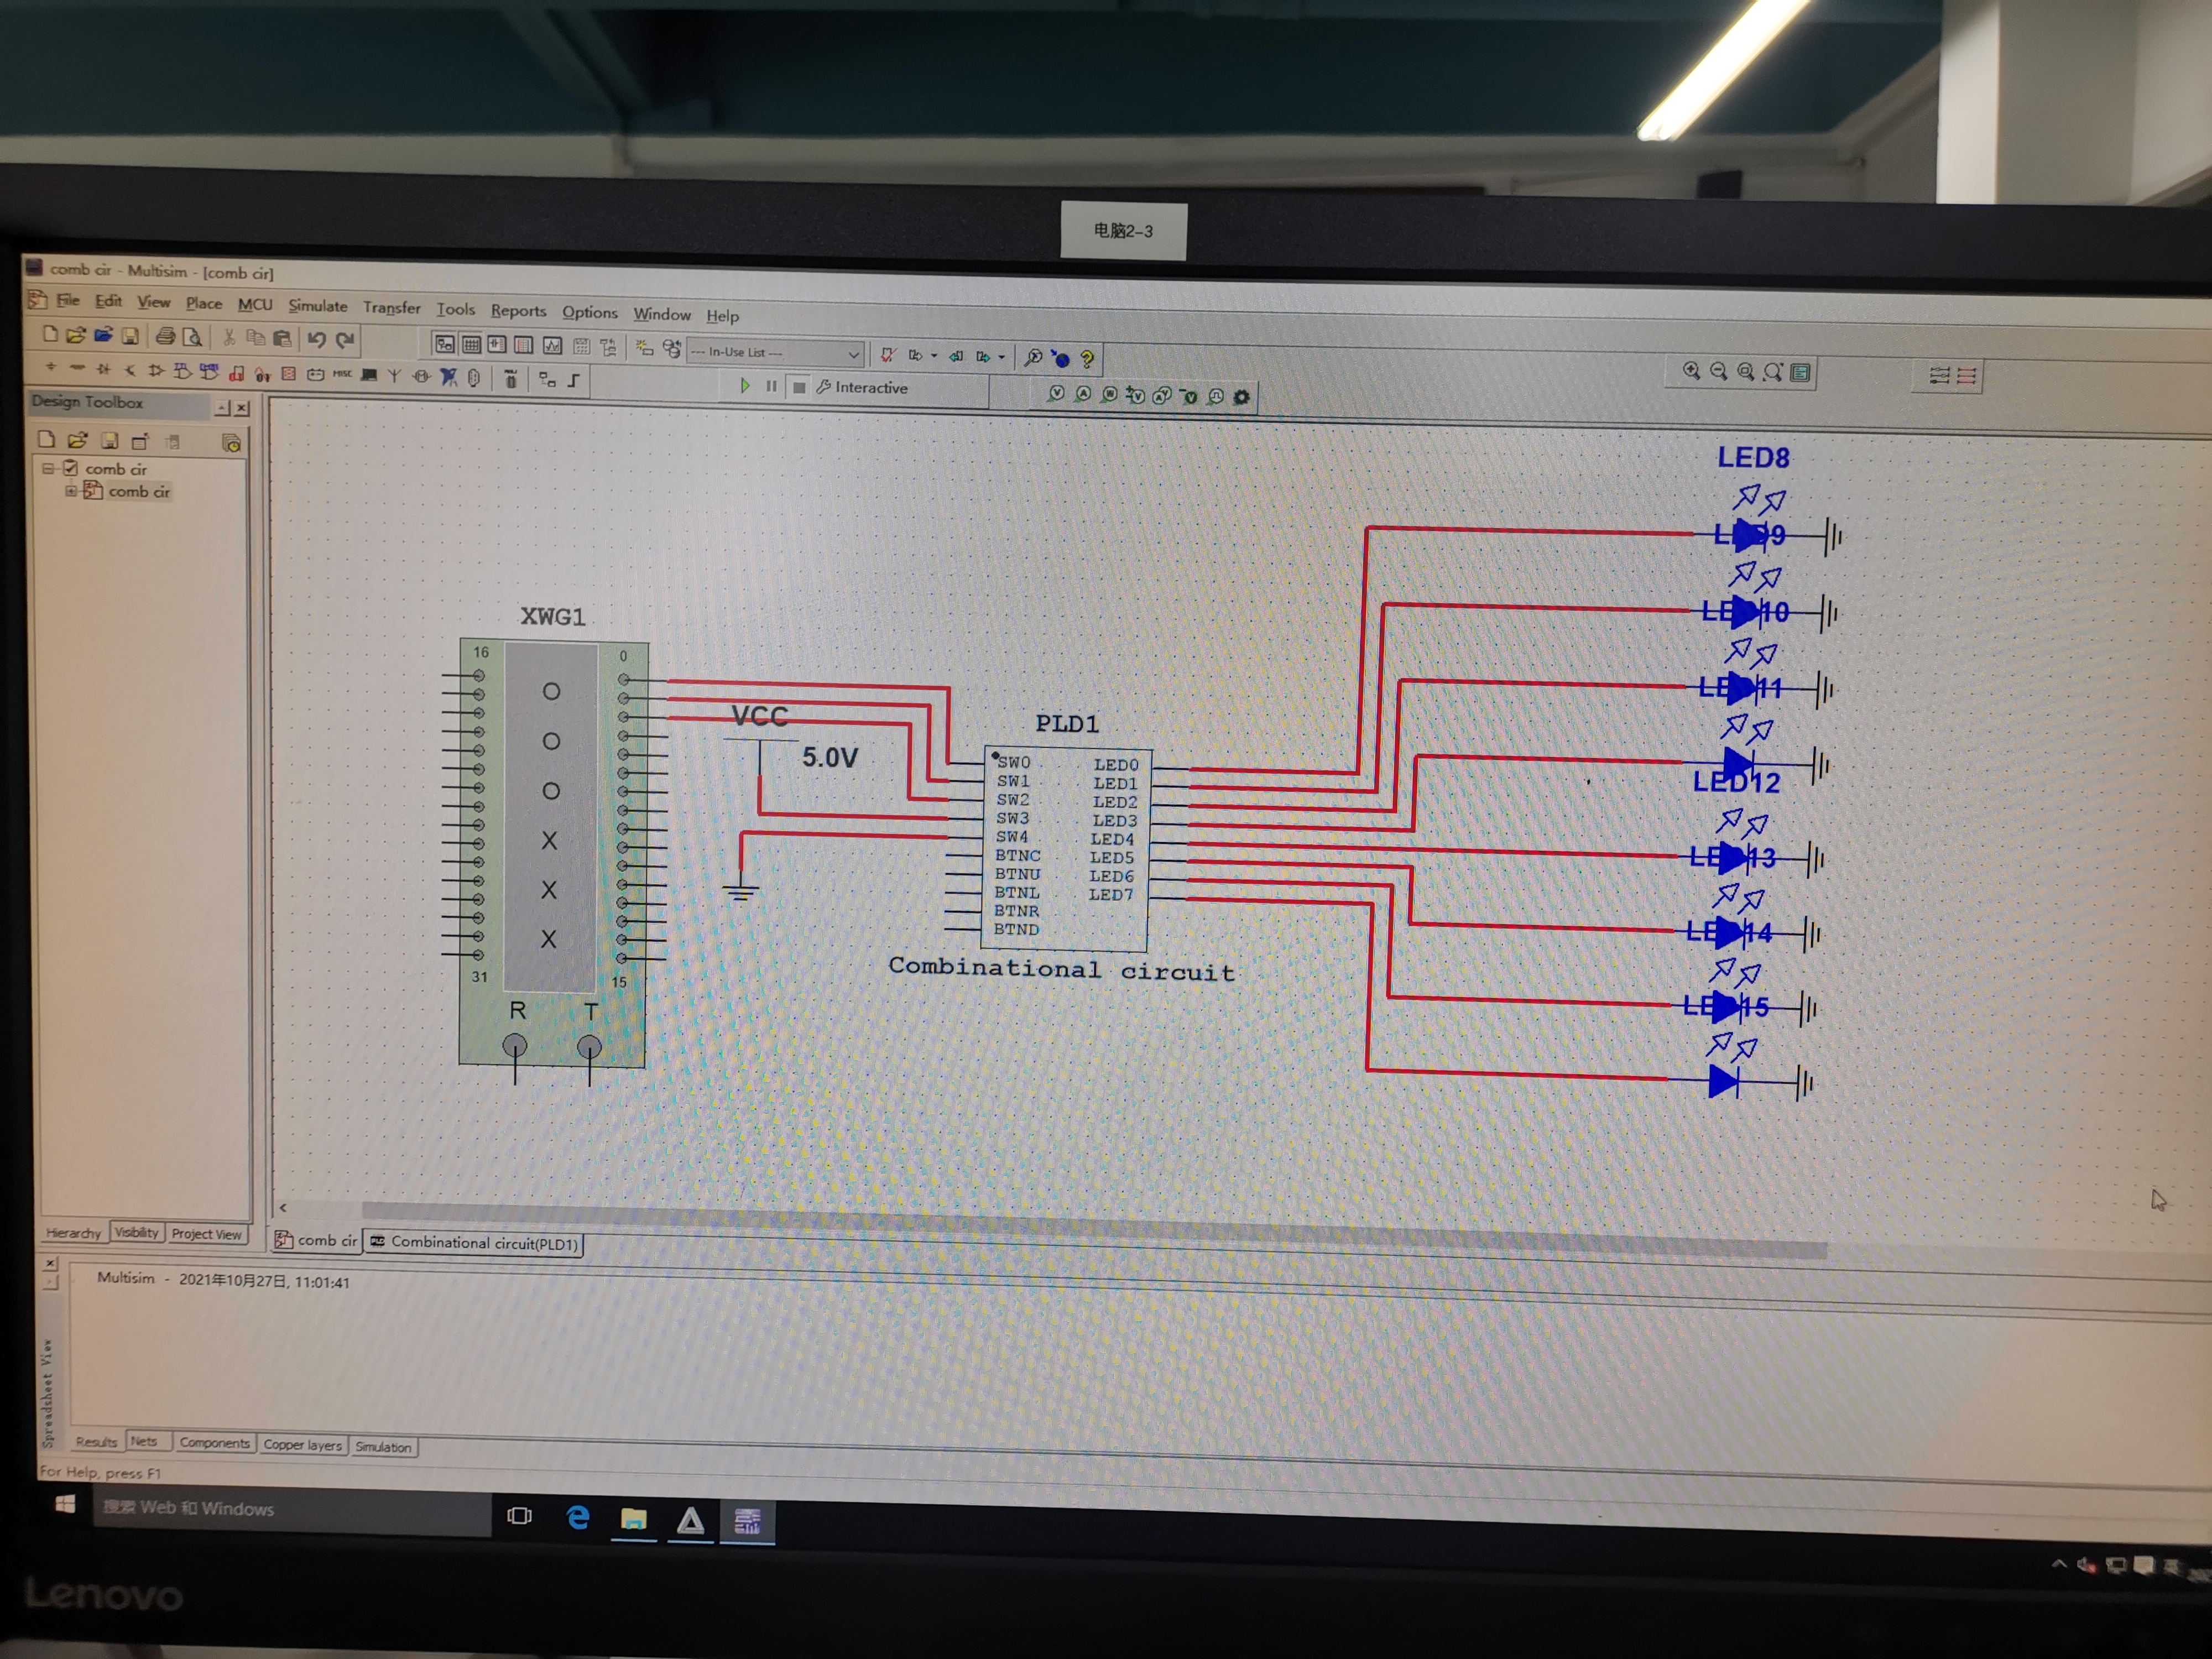
\includegraphics[width=0.8\textwidth]{Original pic/multisim circuit.jpg}
    \end{center}
    \caption{multisim仿真电路}
    \label{multisim circuit}
\end{figure}

\par 仿真功能验证完成后,将电路比特流文件下载到开发板,进行验证。

\subsubsection{实验结果}
\par 各输入状态下电路的输出结果如图\ref{38dec}所示。

\begin{figure}[H]
    \centering
    \subfigure[000]{
    \includegraphics[width=0.3\textwidth]{Original pic/000.jpg}}
    \subfigure[001]{
    \includegraphics[width=0.3\textwidth]{Original pic/001.jpg}}
    \subfigure[010]{
    \includegraphics[width=0.3\textwidth]{Original pic/010.jpg}}
    \subfigure[011]{
    \includegraphics[width=0.3\textwidth]{Original pic/011.jpg}}
    \subfigure[100]{
    \includegraphics[width=0.3\textwidth]{Original pic/100.jpg}}
    \subfigure[101]{
    \includegraphics[width=0.3\textwidth]{Original pic/101.jpg}}
    \subfigure[110]{
    \includegraphics[width=0.3\textwidth]{Original pic/110.jpg}}
    \subfigure[111]{
    \includegraphics[width=0.3\textwidth]{Original pic/111.jpg}}
    \subfigure[未使能]{
    \includegraphics[width=0.3\textwidth]{Original pic/not enable.jpg}}
    
    \caption{3-8译码器}
    \label{38dec}
\end{figure}

\subsubsection{小结}
\par 成功地设计并实现了3-8译码器电路,熟悉了从设计到片上部署的流程。


\section{实验小结}
\begin{enumerate}
    \item 验证了组合逻辑电路逻辑运算的关系,实验结果与理论推导相符。
    \item 熟悉了FPGA开发板的使用。
    \item 熟悉了从设计到芯片部署的流程。
\end{enumerate}


\section*{原始数据}

\begin{figure}[H]
    \begin{center}
        \includegraphics[width=0.8\textwidth]{excel.png}
    \end{center}
\end{figure}

\begin{figure}[H]
    \begin{center}
        \includegraphics[width=0.8\textwidth]{sign.pdf}
    \end{center}
\end{figure}


\end{document}